%!TEX root = master.tex


\section{Introduction}

This course bla bla bla

\section{Probability review}
Let first take a look at the \emph{Sample space}: 
\begin{itemize}
    \item Dice: $\Omega$ = \{1,2,3,4,5,6\}
    \item Coin flip: $\Omega$ = \{heads, tails\}
\end{itemize}
There are also \emph{Events} which is a subset of the sample space:
\begin{itemize}
    \item Dice: A = \{ 1,2\}
    \item Coin flip = \{tails\}
\end{itemize}
Three important axioms to remember are.
\begin{enumerate}
    \item P(A) $\ge$ 0
    \item P($\Omega$) = 1
    \item For disjoint sets, $A_1$,$A_2$, $\dots$ \\ $P(A_1 \cup A_2 \cup \dots) = P(A_1) + P(A_2) + \dots$         
\end{enumerate}

To sum it up here are some examples:

\begin{enumerate}
    \item $A \subseteq B \Rightarrow P(A) \le P(B)$
    \item $P(A^{c}) = 1 - P(B)$
    \item $P(\diameter)  = 0$
    \item $0 \le P(A) \le 1$
    \item $P(A \cup B)  = P(A) + P(B) - P(A\cap B)$
\end{enumerate}

\subsection{Conditional probability}
The \textcolor{red}{definition} of conditional probability for two events are the following:

\begin{equation}
    P(B|A) = \frac{P(A \cap B)} {P(A)} 
\end{equation}

Provided that the probability of event A is greater than 0, $P(A) > 0$.
From this we can derive the \textbf{product rule:} $P(A \cap B) = P(B|A)P(A)$


\subsection{Bayes theorem}
Given two events called A and B:

\begin{equation}
    P(B|A) = \frac{P(A|B)P(B)} {P(A)} 
\end{equation}

\begin{example}{Example: medical test paradox}
    Let's characterize a medical test:
    \begin{itemize}
        \item Sensitivity(True positive rate) = $P(+ | \text{Disease})$
        \item Specificity (True negative rate) = $P(- | \text{No Disease})$
    \end{itemize}
    Then characterize a medical condition in a population:
    \begin{itemize}
        \item Prevalence = "\emph{proportion of a particular population found to be affected by a medical condition.}"
    \end{itemize} 
    \vspace{1em}
    \textbf{Question:} Assume that for a certain disease the Sensitivity is 0.99, Specificity is 0.99 and Prevalence = 0.01
    If you pick someone randomly from the population and test the person for this disease, obtaining a positive
    result. What is the probability of the person actually having the disease?
    \vspace{2em}
    
    Using Bayes theorem:

    \begin{equation}
        P(\text{Disease}|+) = \frac{P(+|\text{Disease})P(\text{Disease})} {P(+)} = \frac{\text{tpr} \cdot p} {P(+)}  
    \end{equation}

    and by the law of total probability: \\
    $P(+) = P(+ \cap \text{Disease}) + P(+ \cap \text{No disease})$ \\
    $P(+) = P(+|\text{disease})P(\text{disease}) + (1-P(-|\text{No disease}))(1-P(disease))$ \\
    $P(+) = \text{tpr} \dot p + (1 - \text{tnr})\dot (1-p)$ \\

    \vspace{2em}

    Hence we have:

    \begin{equation}
        P(disease|+) = \frac{0.99 \cdot 0.01} {0.99 \cdot 0.01 + 0.01 \cdot 0.99} = 0.5
    \end{equation}
\end{example}

\subsection{Random variables}
The definition of a \textcolor{red}{random variable} $\mathcal{X}$ is a quantity that depends on a random event. Where a
\textcolor{red}{discrete random variable} is a countable number of values. Described by the probability mass function 
$p(x) = P(X=x)$. An \textbf{example:} 6-sided dice with $p(x) = 1/6, x=1, \dots, 6$.
A \textcolor{red}{continuous random variable} is an uncountable number of values. Ex: any value in $\mathbb{R}$. \textbf{Example:} $\mathcal{X}$ is the height of an adult randomly sampled from the population.
It is described by the probability density function: $p(x)$.
\newline
A \textcolor{red}{probability density function} $p(x)$ describes the probability for a \emph{continuous} random variable $x$ falling into a given interval:

\begin{equation}
    P(a < X < b) = \int_{a}^{b} p(x)\,\text{d}x
\end{equation}

\begin{figure}[ht!]
\centering
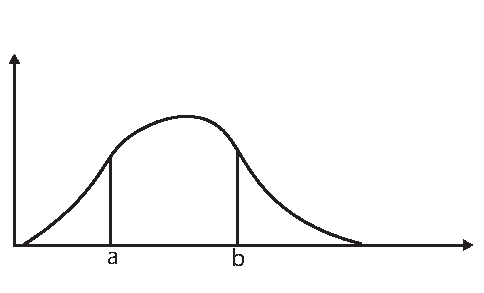
\includegraphics{/Users/linusfalk/Documents/latex/latex_master2_semester3/figures/new-figure-1693205116382.pdf}
\caption{Example of caption}
\label{fig:example}
\end{figure}

\subsection{Joint probability}
Given two random variables: X and Y:

\begin{itemize}
    \item Discrete: probability mass function \\ 
    $p(x,y) = P(X=x, Y = y)$
    \item Continuous: (probability density function) \\
    $P(a < X \le b, c < Y \le d) = \int_{a}^{b}\int_{c}^{d} p(x,y) \,\text{d}y \text{d}x$
\end{itemize}



\subsection{Marginalization and conditioning}
\textbf{Marginalization} (also called the \textbf{sum rule}) is defined as 

\begin{equation}
\begin{aligned}
    p(\textcolor{red}{x}) = \int_{y} p(\textcolor{red}{z},\textcolor{blue}{y}) \,\text{d}\textcolor{blue}{y} \quad \text{if \textcolor{blue}{y} is continuous} \\
    p(\textcolor{red}{x}) = \sum_{\textcolor{blue}{y}}^{} p(\textcolor{red}{x}, \textcolor{blue}{y}) \quad \text{if \textcolor{blue}{y} is discrete}
\end{aligned}
\end{equation}

\textbf{Conditional probability} also called the \textbf{product rule} is defined as:

\begin{equation}
\begin{aligned}
    p(\textcolor{red}{x}, \textcolor{blue}{y}) = \frac{p(\textcolor{red}{x}, \textcolor{blue}{y})} {p(\textcolor{blue}{y})} \quad \text{where} p(\textcolor{blue}{y}) \neq 0  \\
    \Rightarrow p(\textcolor{red}{x}, \textcolor{blue}{y}) = p(\textcolor{red}{x}| \textcolor{blue}{y})p(\textcolor{blue}{y})
\end{aligned}
\end{equation}

\subsection{Bayes theorem: random variables}
Both for probability mass functions and probability density functions:

\begin{equation}
    p(x|y) = \frac{p(y|x)p(x)} {p(y)} 
\end{equation}



\subsection{Probabilistic modelling}
In probabilistic modelling we consider two types of variables:

\begin{equation}
\begin{aligned}
    \textcolor{red}{\mathcal{D} = \{x_1,x_2, \dots, X_N \}: \quad \text{observed variables}} \\ 
    \textcolor{blue}{\Theta = \{x_1,x_2, \dots, X_N \}: \quad \text{latent variables}}
\end{aligned}
\end{equation}

\begin{wbox}{}
    In \textbf{probabilistic modelling} we treat \emph{both} the \textcolor{blue}{observed variables} and the \textcolor{red}{latent variables} as \textbf{random variables} 
\end{wbox}
s0

We model this relationship between $\textcolor{red}{\mathcal{D}}$ and $\textcolor{blue}{\Theta}$ with its \textbf{Joint distribution}

\begin{equation}
    p(\textcolor{blue}{\mathcal{D}}, \textcolor{red}{\Theta}) = p(\textcolor{blue}{x_1, \dots, X_N},\textcolor{red}{z_1, \dots, z_M})
\end{equation}


\subsection{Bayes theorem in Probabilistic modelling}
The joint distribution factorizes into \textbf{likelihood} and a \textbf{prior}

\begin{equation}
    p(\textcolor{blue}{\mathcal{D}}, \textcolor{red}{\Theta}) = p(\textcolor{blue}{\mathcal{D}}|\textcolor{red}{\Theta})p(\textcolor{red}{\Theta}) 
\end{equation}

We can now find $p(\textcolor{red}{\Theta} | \textcolor{blue}{\mathcal{D}})$ using \textbf{Bayes' theorem}

\begin{equation}
    p(\textcolor{red}{\Theta} | \textcolor{blue}{\mathcal{D}}) = \frac{p(\textcolor{blue}{\mathcal{D}}|p(\textcolor{red}{\Theta}))} {p(\textcolor{blue}{\mathcal{D}})} 
\end{equation}


\begin{definition}{}
\begin{itemize}
    \item $\textcolor{blue}{\mathcal{D}}$ : observed data
    \item $\textcolor{red}{\Theta}$ : latent variables explaining the data
    \item $p(\textcolor{red}{\Theta})$ : \textbf{prior} belief of latent variables before seeing data
    \item $p(\textcolor{blue}{\mathcal{D}}|\textcolor{red}{\Theta})$: \textbf{likelihood} of the data in view of the latent variables
    \item $p(\textcolor{red}{\Theta}|\textcolor{blue}{\mathcal{D}})$: \textbf{posterior} belief of latent variables in view of data 
    \item $p(\textcolor{blue}{\mathcal{D}})$: The \textbf{marginal likelihood} (presented in lecture 3)
\end{itemize}
\end{definition}


\begin{example}{Example: Coin flip (Bayesian viewpoint)}
\begin{itemize}
    \item $x \in \{ 0,1\}$ represent the outcome of flipping a damaged coin 
    \item $p(x=1 | \mu) = \mu$ , which is also a random variable. 
    \item Probability distribution $p(\mu)$: our \emph{prior belief} 
\end{itemize}

\vspace{2em}

\textbf{Question:} After we observe $N$ coin flips $\{ x_1, \dots, x_N\}$, what is our belief $p(\mu | x_1, \dots, x_N)$?

\textbf{Solution:} Bayes theorem states that:

\begin{equation}
    p(\mu | x_1, \dots, x_N) \propto p(x_1, \dots, x_N | \mu)p(\mu) 
\end{equation}

We will continue with this example next lecture... 

\end{example}


\subsection{Condluding remarks}
Probabilistic/Bay inference is a flexible way of dealing the machine learning problems. Some properties to remember:

\begin{itemize}
    \item Treat not only the data, but also the model and its parameters (if they are parametric) as random variables
    \item After learning you not only get a single model, you get a distribution of likely models.
    \item You can also encode prior knowledge you might have about the model  and its parameters.
\end{itemize}

\subsection{Summary}
\textbf{Probability distribution} is a function that describes the likelihood of obtaining the possible values that a random variable can assume. \textbf{Conditional and marginalization} are two basic rules for manipulating probability distributions. \textbf{Frequentist vs Bayesian}: the first assume true values underlying some experiment and the second require some initial belief to be set on possible values.

\begin{itemize}
    \item Bayes theorem: $p(x|y) = p(y|x)p(x)/p(y)$
    \item \textbf{Prior}, belief of parameters before we have seen any data
    \item \textbf{Likelihood}, belief of data in view of the parameters
    \item \textbf{Posterior}, belief of parameters after inferring data
\end{itemize}








